% Converted from reference/DB4OFlare (MadCap Flare, Java target)

\chapter{Object Manager Enterprise}
\label{ref:object-manager-enterprise}

Object Manager Enterprise (OME) is an object browser for db4o databases. OME installation can be found in /ome folder of the distribution. The zip file in this folder contains the Eclipse plugin version of OME. To install the plugin, you need to have a version of Eclipse \textgreater{}= 3.3 installed. Unzip the file to a folder of your choice. Then open Eclipse, select 'Help' -\textgreater{} 'Software Updates...' -\textgreater{} 'Available Software' from the menu. Choose 'Add Site...' -\textgreater{} 'Local...' and select the unzipped folder. Follow the Eclipse Update Manager instructions for the OME feature from here on. The actual menu structure may vary over Eclipse versions. (The above applies to Eclipse 3.4 Ganymede.) When in doubt, please refer to the Eclipse documentation on Software Updates. Alternatively, you can install the plugin manually by simply copying the contents of the 'plugins' and 'features' folders from the unzipped folder to the corresponding subfolders in the root folder of your Eclipse installation.

More Reading:

\begin{itemize}
\item \hyperref[ref:object-manager-enterprise-ome-for-eclipse-ome-interface]{OME Interface} (p.~\pageref{ref:object-manager-enterprise-ome-for-eclipse-ome-interface})
\item \hyperref[ref:object-manager-enterprise-ome-for-eclipse-browsing-a-database]{Browsing A Database} (p.~\pageref{ref:object-manager-enterprise-ome-for-eclipse-browsing-a-database})
\item \hyperref[ref:object-manager-enterprise-ome-for-eclipse-querying]{Querying} (p.~\pageref{ref:object-manager-enterprise-ome-for-eclipse-querying})
\end{itemize}

\section{OME Interface}
\label{ref:object-manager-enterprise-ome-for-eclipse-ome-interface}

Once the Object Manager (OM) is installed you can see it in Eclipse by selecting Window-\textgreater{}Open Perspective-\textgreater{}Other and choosing "OME". Typically, OME window should look similar to this:

\begin{center}
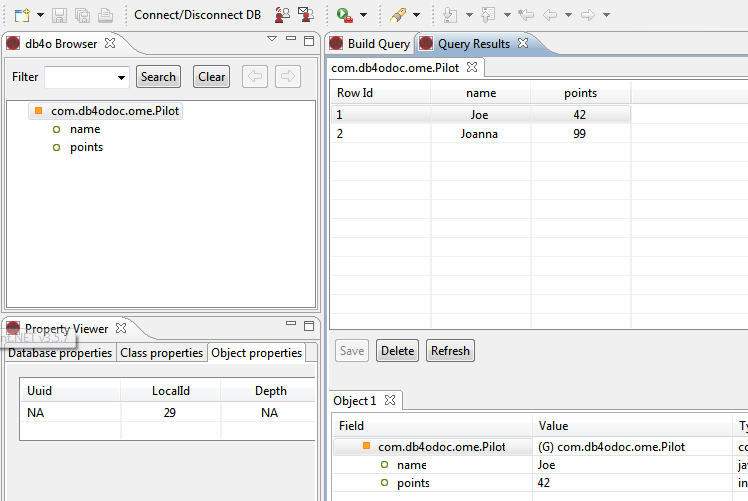
\includegraphics[width=\maxwidth]{images/ref-object-manager-enterprise-ome-for-eclipse-ome1.png}
\end{center}
In the OME perspective you can see:

\begin{itemize}
\item OME menu:

\begin{center}
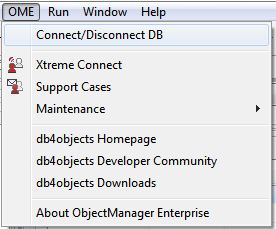
\includegraphics[width=\maxwidth]{images/ref-object-manager-enterprise-ome-for-eclipse-ome-menu.png}
\end{center}
\item OME toolbar buttons to access the frequently used functionality fast
\item Db4o Browser: window displaying the contents of the open db4o database
\item Property Viewer: window displaying the properties of the open database or the properties of the selected database class
\item Build Query: windows allowing to build a query using drag\&drop functionality
\item Query Results: window to browse the results of the query execution
\end{itemize}

\section{Browsing a Database}
\label{ref:object-manager-enterprise-ome-for-eclipse-browsing-a-database}

Suppose you have a simple database file containing Pilot and Car objects. Please select OME-\textgreater{}Connect/Disconnect DB (or use a shortcut button from the toolbar menu) and browse to your database file.

Once you've connected you will see a screen similar to this:

\begin{center}
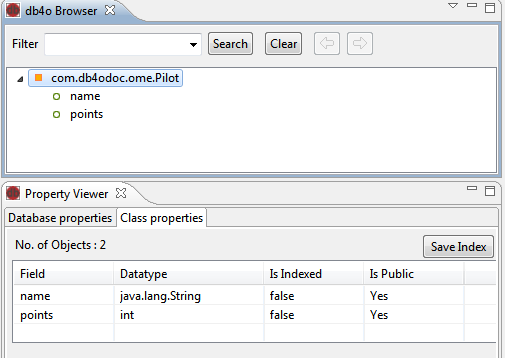
\includegraphics[width=\maxwidth]{images/ref-object-manager-enterprise-ome-for-eclipse-ome-pilot.png}
\end{center}
The db4o Browser window in the picture above shows that there is 1 class in the database (Pilot), which contains 2 fields: name and points. In the Property Viewer you can see more information about the class fields. You can also change "Is indexed" field and add the index to the database by pressing "Save Index" button.

The filter panel on the top of the view allows easier navigation through the database with lots of different classes. You can use wildcard searches and benefit from the search history to make the selection faster.

\section{Querying}
\label{ref:object-manager-enterprise-ome-for-eclipse-querying}

It is easy to retrieve all of the Pilot instances from the database: just right-click the Pilot class in db4o Browser and select "View All Objects". The list of the Pilot objects will be shown in the Query Result view:

\begin{center}
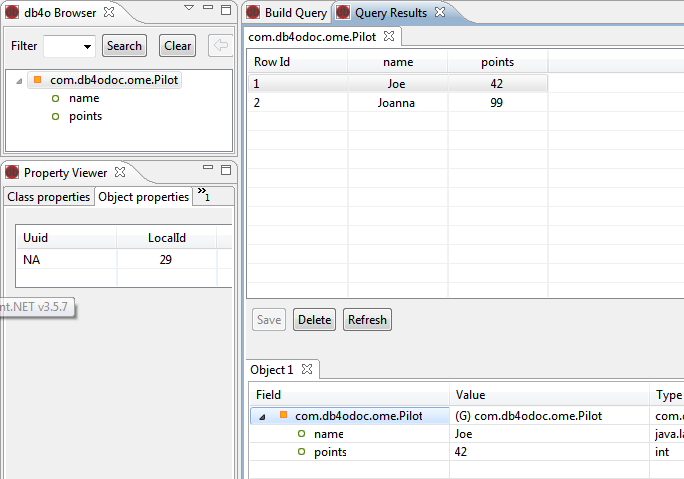
\includegraphics[width=\maxwidth]{images/ref-object-manager-enterprise-ome-for-eclipse-ome-result.png}
\end{center}
You can see object details in the detailed view below. Try to change any values and use Save button to persist the changes to the database. You can also use Delete button to delete objects from the database. For the objects containing field objects you will be prompted to use cascade on delete.

More complex queries can be done by using Build Query view:

\begin{center}
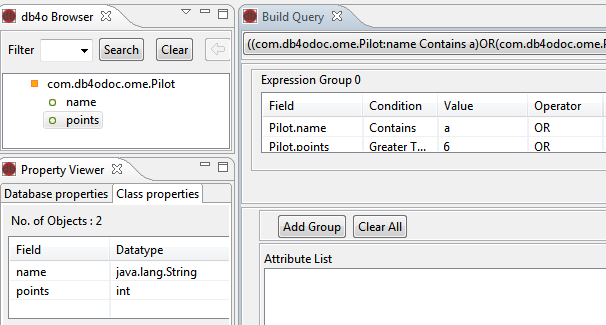
\includegraphics[width=\maxwidth]{images/ref-object-manager-enterprise-ome-for-eclipse-ome-query.png}
\end{center}
Drag "points" field from the db4oBrowser view into the Build Query view, set condition "Greater Than", put a value "99" and run the query. You can return to the Built Query tab and modify the query later on again. For example: add "AND" operator, drag "name" field and set the value to "Michael Schumacher". Re-run the query.

When the new query is created, the previous query is stored and can be selected from the history drop-down:

\begin{center}
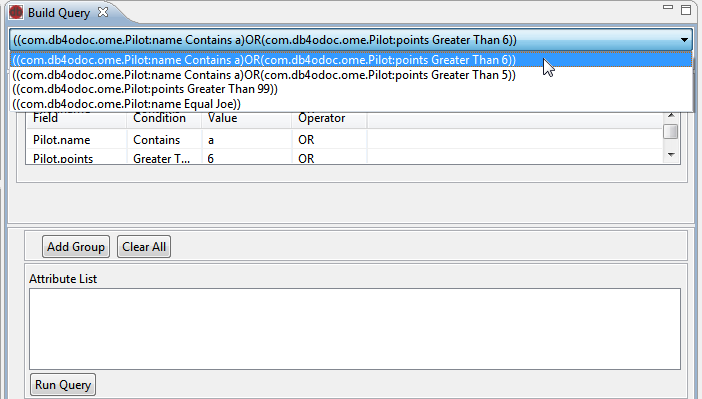
\includegraphics[width=\maxwidth]{images/ref-object-manager-enterprise-ome-for-eclipse-ome-qhistory.png}
\end{center}
More sophisticated queries can be build by joining grouped constraints using "Add Group" button.

When you are done working with the database in OME, you can close the connection by using OME-\textgreater{}Connect/Disconnect DB menu command or by using the equivalent button on the toolbar.

\section{Custom Configuration}
\label{ref:object-manager-enterprise-ome-for-eclipse-custom-config}

When the database cannot be opened with OMJ you should try to pass your configuration to OMJ. This ensures that OMJ opens the database the same way as your application does.

\subsection*{Prepare Configuration Jar File}

First you need to prepare a jar-file which contains code to configure OMJ. You do this by implementing the EmbeddedConfigurationItem-interface or implementing ClientConfigurationItem-interface.

In the implementation you can apply all the configuration settings to the object container which you use in your application.

\begin{lstlisting}
public class ConfigureDBForOmj implements EmbeddedConfigurationItem{
    public void prepare(EmbeddedConfiguration embeddedConfiguration) {
        // Your configuration goes here.
        // For example:
        embeddedConfiguration.common().add(new UuidSupport());
    }

    public void apply(EmbeddedObjectContainer embeddedObjectContainer) {
    }
}
\end{lstlisting}

{\small\itshape ConfigureDBForOmj.java: A configuration item for Java\par}
\medskip

Then create the file 'com.db4o.config.EmbeddedConfigurationItem' in the 'META-INF/services' folder of your jar. Add the fully qualified name of your EmbeddedConfigurationItem/ClientConfigurationItem-implementation. You can list as many implementations as you want.

\begin{lstlisting}
com.db4odoc.omj.ConfigureDBForOmj
\end{lstlisting}

{\small\itshape com.db4o.config.EmbeddedConfigurationItem: List all configuration items for OMJ\par}
\medskip

Finally you need to package the compiled code and the 'META-INF/service' folder into a jar-file. The jar-layout should be like this:

\begin{center}
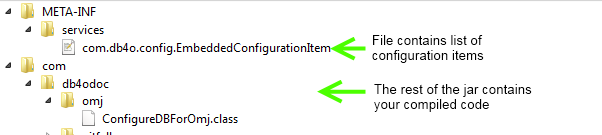
\includegraphics[width=\maxwidth]{images/ref-object-manager-enterprise-ome-for-eclipse-jar-overview.png}
\end{center}
\subsection*{Using the Configuration in OMJ}

After that you can choose the 'Custom config...' option on the open-dialog. There add the jar-file you've build previously. On the right all configuration-items are listed. Select the appropriate configuration items for your database.

\begin{center}
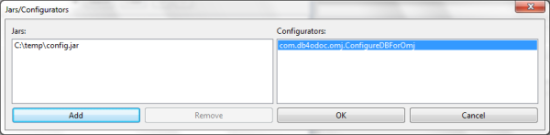
\includegraphics[width=\maxwidth]{images/ref-object-manager-enterprise-ome-for-eclipse-custom-config.png}
\end{center}
\section{Problems?}
\label{ref:object-manager-enterprise-ome-for-eclipse-problems}

Are you experiencing problems with the object manager? You can take a look at the error log in the Eclipse workspace. The log is located here: "workspace/.metadata/.log". Maybe you need to first clean up the log and then reproduce the issue.

When you are using advanced configuration features like type handlers, special string encoding etc. you should \hyperref[ref:object-manager-enterprise-ome-for-eclipse-custom-config]{add your configuration} (p.~\pageref{ref:object-manager-enterprise-ome-for-eclipse-custom-config}) to the object manager.

Otherwise ask for help in the \href{http://community.versant.com/Forums.aspx}{db4o forums}. When you see errors in the log please include them in your post.

